%pracu piseme dvoma farbami:
%ciernou piseme veci, ktore vedia citatela
%modrou detaily
%Matici sa staruju len aby predali spravnost, Informatici aj motivaciu.

%\documentclass[12pt,a4paper,twoside]{report}
\documentclass[12pt,a4paper]{article}


\usepackage[slovak]{babel}
\usepackage[utf8]{inputenc}
\usepackage{a4wide}
\usepackage{tabularx}
\usepackage{amsfonts}
\usepackage{amssymb}
\usepackage{amsmath}
\usepackage{epsfig}
\usepackage{color}
\usepackage{mathrsfs}
\usepackage{verbatim}
\usepackage{hyperref}
\usepackage{subfigure}
\usepackage{float}
\usepackage{longtable}
\usepackage{listings}
\usepackage{multicol}
\usepackage{graphicx}
\usepackage{pdfpages}
\usepackage{lastpage}
\usepackage{fancyhdr}
\usepackage{url}
\usepackage[small,bf]{caption}
\usepackage[T1]{fontenc}   

                                  
\hypersetup{%  http://www.tug.org/applications/hyperref/
    bookmarksnumbered,
    pdfstartview={FitH},
    %linkcolor=black,
    %citecolor=black,
    colorlinks=true
}

\let\stdsection\section{}
\renewcommand\section{\newpage\stdsection}

%%%%%%%%%%%%%%%%%%%%%%%%% CUSTOMIZACIA BEGIN %%%%%%%%%%%%%%%
\setlength{\textheight}{24cm}
\setlength{\textwidth}{15.5cm}
\addtolength{\voffset}{-1.2cm}
\addtolength{\hoffset}{0.0cm}
\setlength{\parindent}{0.5cm}
\setlength{\parskip}{0in}
\setlength{\headheight}{16pt}
\linespread{1.5}

\hypersetup{
    colorlinks=true,       % false: boxed links; true: colored links
%    linkcolor=black,          % color of internal links
%    citecolor=black,        % color of links to bibliography
%    urlcolor=black,           % color of external links
%    linkbordercolor=black, % 	color of frame around internal links (if colorlinks=false)
%    citebordercolor=black, %	color of frame around citations
%    urlbordercolor=black, %	color of frame around URL links
}

%\setlength{\topmargin}{-10mm}
%\setlength{\textwidth}{16truecm}
%\setlength{\textheight}{24truecm}
%\setlength{\oddsidemargin}{0mm}
%\setlength{\evensidemargin}{0mm}
%%%%%%%%%%%%%%%%%%%%%%%%% CUSTOMIZACIA END %%%%%%%%%%%%%%%

\begin{document}

\setcounter{page}{1}
\pagenumbering{roman}
\thispagestyle{empty}

    \begin{center}
    \large{
        \textbf{
            UNIVERZITA KOMENSKÉHO V BRATISLAVE \\ 
            FAKULTA MATEMATIKY, FYZIKY A INFORMATIKY
        }
    }
\end{center}

\vspace{2cm}

\begin{figure}[!h]
    \centering
    
\includegraphics[width=3.5cm]{img/komlogo-new}
\end{figure}

\vspace{1cm}

\begin{center}
    \large{
        \textbf{
            ANALYSIS OF THE GENERALIZED \\
            RECIRCULATION-BASED LEARNING ALGORITHM \\
            IN BIDIRECTIONAL NEURAL NETWORK \\
            \vspace{3cm}
            DIPLOMA THESIS
        }
    }
\end{center}

\vfill

\begin{multicols}{2}
    \begin{flushleft}
        \textbf{2012}
    \end{flushleft}
    \begin{flushright}
        \textbf{Peter CSIBA}
    \end{flushright}
\end{multicols}

    
\newpage
\thispagestyle{empty}
%\addtolength{\hoffset}{4mm}
%\setlength{\oddsidemargin}{-5mm}
%\setlength{\evensidemargin}{5mm}

    \begin{center}
    \large{
        \textbf{
            UNIVERZITA KOMENSKÉHO V BRATISLAVE \\ 
            FAKULTA MATEMATIKY, FYZIKY A INFORMATIKY
        }
    }
\end{center}


\vspace{5cm}

\begin{center}
    \large{
        \textbf{
            ANALYSIS OF THE GENERALIZED \\
            RECIRCULATION-BASED LEARNING ALGORITHM \\
            IN BIDIRECTIONAL NEURAL NETWORK \\
            \vspace{3cm}
            DIPLOMA THESIS
        }
    }
\end{center}

\vfill

\begin{center}
    \begin{tabular}{ll}
        Študijný program:               &   Informatika \\
        Študijný odbor:                 &   TODO \\
        Školiace pracovisko:            &   Centre for Cognitive Science, Department of Applied Informatics \\
        Školiteľ:                       &   doc. Ing. Igor Farkaš, PhD. \\
    \end{tabular}
\end{center}

\vfill

\begin{multicols}{2}
    \begin{flushleft}
        \textbf{Bratislava 2012}
    \end{flushleft}
    \begin{flushright}
        \textbf{Peter CSIBA}
    \end{flushright}
\end{multicols}

    
\newpage
\thispagestyle{empty}

    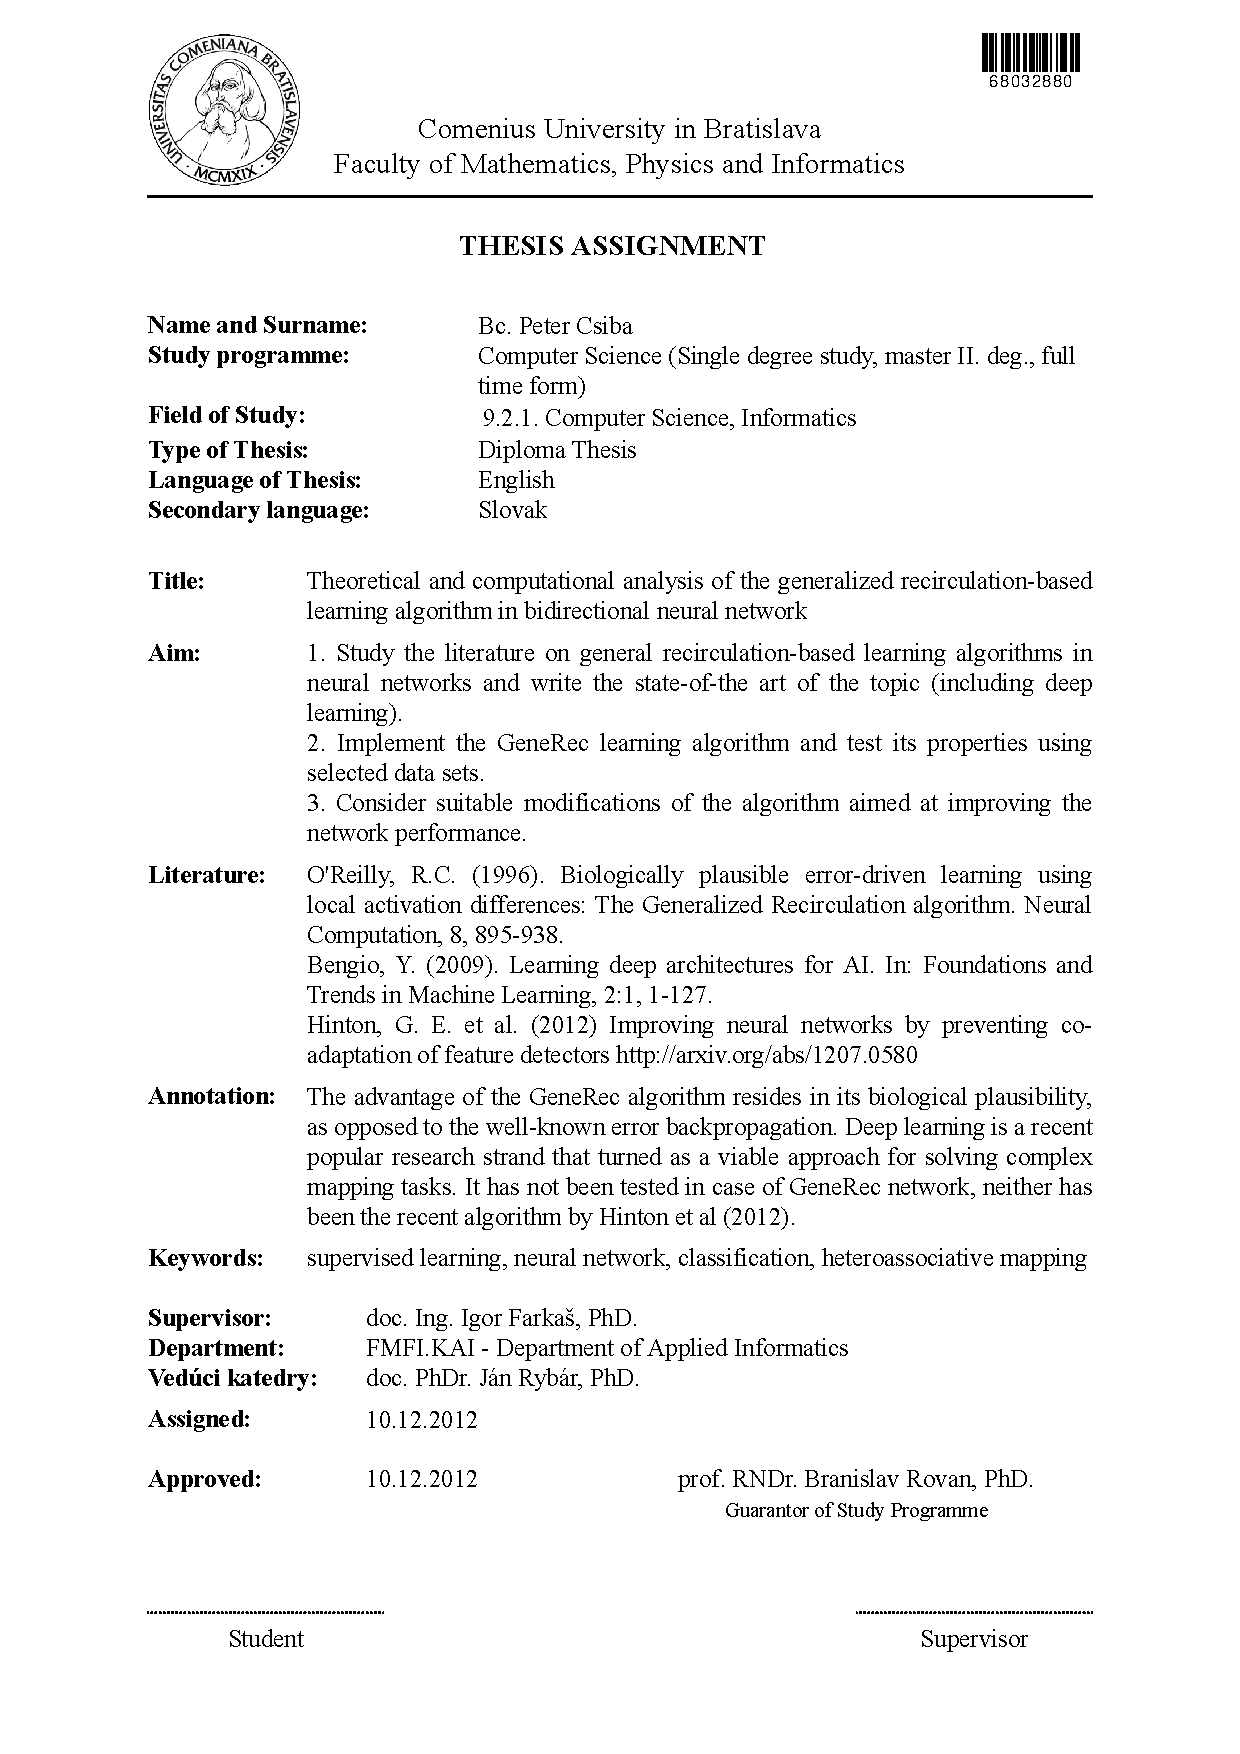
\includepdf[offset=0 -25mm]{img/zadanie_en.pdf}


\newpage
%\thispagestyle{empty}
\thispagestyle{plain}

    \section*{Poďakovanie}



\newpage
%\thispagestyle{empty}

    %Abstract is very important part of the thesis. It will be most read by people and should be written with a great care. The abstract should mention:
% 1) About the problem you want to solve
% 2) About your solution – how you solve the problem
% 3) Highlights about how good is your solution (e.g. achieves 70\% better performance) referring to the results you obtained in your experiments (e.g. achieves 70\% better performance).
% 4) Possible impacts of your work into the field (e.g. “The proposed solution can be used to offload the CPU by executing data parallel computation intensive code on GPUs and thus obtaining additional Speedup for no cost”).

\section*{Abstrakt}
Táto práca pomocou výpočtových simulácií analyzuje umelé neurónové siete (UNS), ktoré sú založené na Generalized recirculation algorithm (GeneRec)~\citep{o1996bio} a Bidirectional Activation-based Learning algorithm (BAL)~\citep{farkas2013bal}. Od štandardných sietí, akými sú napríklad siete spätne šíriace chybu (BP), sa líšia tým, že zmena váh je založená na rozdiely dopredných a spätných aktivácií. Takéto siete sa považujú za prirodzené pre ich obojsmernosť a preto, lebo šíria iba aktiváciu a nie chybu. Je známe, že tieto siete majú problémy s naučením sa aj jednoduchých úloh, ktoré sa BP vie naučiť. Cieľom práce je preto zvýšenie úspešnosti BALu. 

Analyzujeme viacero modifikácií BALu. Na základe pozorovaní navrhujeme model Two learning rates (TLR), ktorý využíva rozdielne rýchlosti učenia pre rôzne matice. Pomocou simulácií potvrdíme, že TLR značne zvyšuje úspešnosť BALu vo viacerých úlohách. Navyše, pozorujeme jasné závislosti medzi rýchlosťami učenia a úspešnosťou siete. Zaujímavosťou je, že pre najlepšie siete môže byť podiel medzi dvoma rýchlosťami učenia až $10^6$. Myšlienku TLR aplikujeme aj na GeneRec. Navyše, skúšame viacero štandardných modifikácií UNS, ako sú napríklad moment, dávkové učenie, dynamická rýchlosť učenia alebo inicializácia váh. 

Veríme, že aplikácia myšlienky TLR má potenciál zvýšiť úspešnosť aj iných modelov UNS. Myšlienka sa dá zovšeobecniť aj na iné parametre, ako sú napríklad moment alebo inicializácia váh. 

\begin{flushleft}
  {\bf Kľúčové slová}: učenie s učiteľom, neurónová sieť, heteroasociatívne zobrazenie, dynamická rýchlosť učenia, učenie na základe aktivácií
\end{flushleft}

%keywords={ Internet; TCP streams; Tor network;}


\newpage
%\thispagestyle{empty}

    %Abstract is very important part of the thesis. It will be most read by people and should be written with a great care. The abstract should mention:
% 1) About the problem you want to solve
% 2) About your solution – how you solve the problem
% 3) Highlights about how good is your solution (e.g. achieves 70\% better performance) referring to the results you obtained in your experiments (e.g. achieves 70\% better performance).
% 4) Possible impacts of your work into the field (e.g. “The proposed solution can be used to offload the CPU by executing data parallel computation intensive code on GPUs and thus obtaining additional Speedup for no cost”).

\section*{Abstract}

% 1) About the problem you want to solve
In our work, we used computational simulations to analyse supervised artificial neural networks based on the Generalized recirculation algorithm (GeneRec) by~\citet{o1996bio} and the Bidirectional Activation-based Learning algorithm (BAL) by~\citet{farkas2013bal}. The main idea of both algorithms is to update weights based on the difference between forward and backward propagation of neuron activations rather than based on error backpropagation (BP) between layers, which is considered biologically implausible. However, both algorithms struggle to learn low dimensional mappings which could be easily learned by BP. The aim of this work is to fill this gap. 

% 2) About your solution – how you solve the problem
Several modifications of BAL are proposed and after systematic analysis a Two learning rates (TLR) version is introduced. TLR uses different learning rates for different weight matrices. The simulations prove increase in success rate and show smooth relation between success and learning rates. For the networks with highest success rate the two learning rates can be in ratio $10^6$. Further the idea of TLR is applied to GeneRec. Finally, additional experiments for momentum, weight initialization, hidden activations and dynamic learning rate are analysed. 

% 4) Possible impacts of your work into the field (e.g. “The proposed solution can be used to of
We believe that using the idea of TLR could lead to performance increase in other artificial neural network models as well, and even multi-layered networks. Intuitively, an increase in success rate could be achieved by generalizing the idea of TLR to additional parameters, such as momentum or weight initialization. Further experiments are outlined. 

\begin{flushleft}
  \textbf{Keywords:} supervised learning, artificial neural network, heteroassociative mapping, dynamic learning rate, activation based learning. 
\end{flushleft}

%keywords={ Internet; TCP streams; Tor network;}


    
\newpage
\setcounter{page}{1}
\pagenumbering{arabic}
\pagestyle{fancy}

\tableofcontents

%    \listoffigures
%    \listoftables
    
\newpage
    
    \section*{Introduction}
\markboth{INTRODUCTION}{}    
\addcontentsline{toc}{section}{Introduction}

Excuse me for my english. Thank you. 

All what is copied from articles is cited. 
%%%%%%%%%%%%%%%%%%%%%%%%%%%%%%%%%%%%%%%%%%%%%%%%%%%%%%%%%%%%%%%%%%%%%%%%%%%%%%%%%%%%


%%%%%%%%%%%%%%%%%%%%%%%%%%%%%%%%%%%%%%%%%%%%%%%%%%%%%%%%%%%%%%%%%%%%%%%%%%%%%%%%%%%%
%\paragraph*{Motivácia}


%%%%%%%%%%%%%%%%%%%%%%%%%%%%%%%%%%%%%%%%%%%%%%%%%%%%%%%%%%%%%%%%%%%%%%%%%%%%%%%%%%%%
%\para*{Členenie práce} 


    
\newpage
    
    \section{Overview of Neural Nets}

\subsection{Motivation}

\paragraph{Feature detector.}
Neural networks have proven their quality as feature detectors of statistical sets. They can extract and create features which represent individual inputs. This is mostly used in image recognition. 

\paragraph{Autoencoder.}
The purpose of an encoder network is to learn good \textit{codes} in the intermediate, hidden units. If for, example, there are less hidden units than input units, an encdoer network will perform data-compression  \cite{hinton1988learning}. Autoencoder is also called autoassociator \cite{bengio2009learning}.

\paragraph{Classifier.}
Aim of classification tasks is to classify individul inputs into a finite number of classes. For example classifying medical results into positive or negative. 

\paragraph{Principal component analysis.}
Goal of PCA analysis is to get main components which can be lineary combined to individual parts of the original image. The resulting components can be treated as features or used for compression. 

\subsection{Standard notation}

\paragraph{Network.}
In general we can define a neural network as a directed weighted graph. Each \emph{unit} (vertex) has its \emph{activation} and usually it changes in discrete time. The \emph{state} of a neural network are current \emph{weights} of edges and current activations. 

\paragraph{Net inuput.}
Each unit $i$ has its \emph{net input} $\eta_i$ defined as:
$$\eta_i = \sum_j w_{ji}x_j,$$
where $w_{ji}$ is the weight of edge from unit $j$ to unit $i$ and $x_j$ is the activation of unit $j$.

\paragraph{Activation.}
Usually the activation of unit $i$ is computed as:
$$x_i = \sigma(\eta_i),$$
where $\sigma$ is a bounded\footnote{
Usually in bounds of interval [0,1].
} nonlinear monotonic differentiable function. In most cases the logistic function is chosen:
$$\sigma(x) = \frac{1}{1 + e^{-x}}.$$

\paragraph{Error function.}
Error function express how much the output of the neural network differs from the \emph{target} output\footnote{
So it should have a lower bound. 
}. The most simple error function is the quadratic error function:
$E = \sum_j \frac{1}{2}(t_j-y_j)^2,$
where $y_j$ are the activations on output units and $t_j$ are the target values.

\paragraph{Learning rule.}
As soon as the error function is defined for the network we can derive an easy rule which applies gradient descent: 
$$\frac{\delta E}{\delta w_{ji}}$$
for each weight. The learning rule describes how to change weights to decrease the error functions.

\paragraph{Input layer.}
Subset of units on which the input values are \emph{clamped}. If the input value for unit $x_i$ is $s_i$ then the activation for unit $x_i$ is simply $s_i$. 

\paragraph{Output layer.}
Similary as the input layer, output layer is a subset of units which activations we treat as the output. 

\paragraph{Hidden layer.}
Set of units which are both not input or output. 

\paragraph{Treshold unit.}
Threshold unit $\theta$ is a form of bias. We can see it as an activator. If the treshold value is high then the activity of the corresponding unit is high and if the treshold value is low then the activity of the corresponding unit is low. 

The treshold term can be elimated by giving every unit an extra input connection whose activity level is fixed at 1. The weight on this special connection is the negative of the treshold, and it can be learned in just the same way as the other weights  \cite{hinton1988learning}.

This method is usually assumed in all papers. 

\paragraph{Training.}
We \emph{train} neural networks on \emph{training sets} of input-output data. For each input we calculate the activation on output layer and compute the error with our error function. Then we apply the learning rule on all weights. This way we iterate through the whole training set. One \emph{epoch} is one iteration through all training values. We repeat training for dozens of epoch with respect to the error function. \emph{Over-fitting} and \emph{under-fitting} must be taken into account.   

\paragraph{Batch update.}
Instead of updateing the weights after activation of each input, the weight changes are accumulated and weights are updated only after all the inputs were fed into the network. 



\subsection{Existing models}

In this section we list models which are similar to GeneRec model. We aim for inspiration and similarities. 

\input{models-bp}

\input{models-ap}

\input{models-recirc}

\input{models-boltzmann}

\input{models-chl}

\input{models-deep}

\subsubsection{Other}
TODO





\subsection{GeneRec}

Generec stands for Generalized Recirculation \cite{o1996bio}\cite{o1996leabra}.

\subsubsection{Model}
%Todo copy from the article

\subsubsection{Attributes and Applications}
%Todo copy from the article






\newpage

\section{Our Research} 

\subsection{Our Motivation}
\cite{o1998six}
O'Reilly presents what he thinks as biologically plausible. In the end of this review we provide citations from this article which shortly explain the most important concepts of NN design. 

Article also contains interesting references to several experiments. It also presents the Leabra model (PhD thesis of O'Reilly) which is presented as a base model for other NN which can be derived from Leabra. The question how to merge the proposed principles is dicussed, especially the case of competiveness and distributed representation. 

Biological realism. "Moreover, computational mechanisms that violate
known biological properties should not be relied upon. "

Distributed representations. "A distributed representation
uses multiple active neuron-like processing units to encode
information (as opposed to a single unit, localist represen-
tation), and the same unit can participate in multiple repre-
sentations. Each unit in a distributed representation can be
thought of as representing a single feature, with information
being encoded by particular combinations of such features.
"

Inhibitory competition. " Inhibitory competition arises when mutual
inhibition among a set of units (i.e. as mediated by in-
hibitory interneurons) prevents all but a subset of them
from becoming active at a time.  Furthermore, most learn-
ing mechanisms (including those discussed later) are
affected by this selection process such that only the selected
representations are refined over time through learning, re-
sulting in an effective differentiation and distribution of
representations. More generally, it seems as though the world can be usefully
represented in terms of a large number of categories with a
large number of exemplars per category (animals, furniture,
trees, etc.). "

Bidirectional activation propagation (interactivity). "They showed that
interactivity could explain the counterintuitive finding that
higher-level word processing can influence lower-level letter
perception. More recently, Vecera and O’Reilly showed
that bidirectional constraint satisfaction can model people’s
ability to resolve ambiguous visual inputs in favor of familiar
versus novel objects. "

Error-driven task learning. "Error-driven learning (also called ‘supervised’ learning) is
important for shaping representations according to task de-
mands by learning to minimize the difference (i.e. the error)
between a desired outcome and what the network actually
produced. "

Hebbian model learning. "that something like correlational structure is important.
Hebbian learning mechanisms represent this correlational
structure, encoding the extent to which different things co-
occur in the environment."

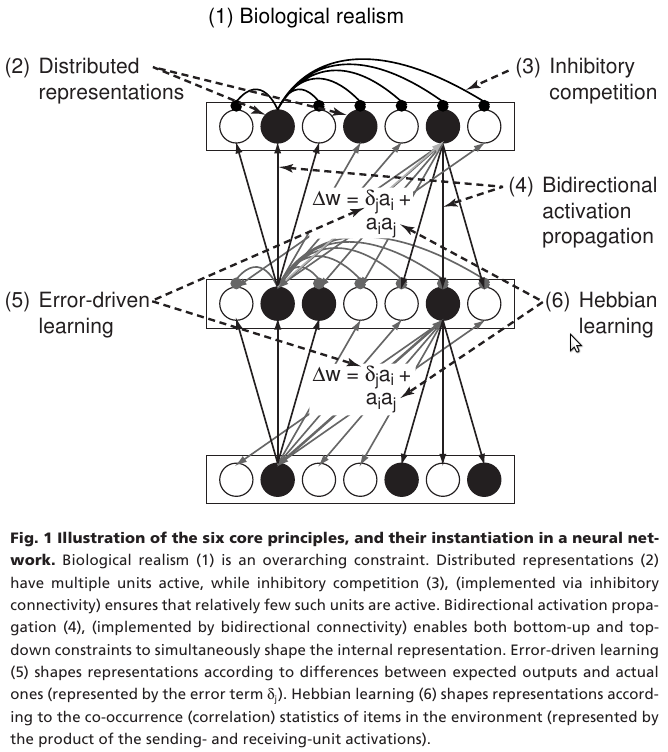
\includegraphics[width=12cm]{img/bio_plausability_o1998six.png}


\newpage

%Implementation – in implementation section you should mention the tools that you use to implement, the target environment (e.g. linux, windows). Limitations (e.g. buffer sizes, connections number).

\section{Implementation} 




 
   
\newpage
    
    \section*{Conclusion}
\markboth{CONCLUSION}{}
\addcontentsline{toc}{section}{Conclusion}

Many work should be done. 



    
\newpage
    
    \section*{Dictionary}
\markboth{DICTIONARY}{}    
\addcontentsline{toc}{section}{Dictionary}

\begin{itemize}
\item Differential equations - TODO learn the basics (to have an intuition for computing the learning rules). Continuous? Ask Ondrac for materials. 
\item Difference equations - TODO learn the basics (to have an intuition for computing the learning rules). Discrete? 
\item Antiparallel vectors - (Wiki, TODO) In a vector space over $\mathbb{R}$ (or some other ordered field), two nonzero vectors are called antiparallel if they are parallel but have opposite directions. In that case, one is a negative scalar times the other.
\item Kronecker delta - (Wiki, TODO) In mathematics, the Kronecker delta or Kronecker's delta, named after Leopold Kronecker, is a function of two variables, usually integers. The function is 1 if the variables are equal, and 0 otherwise: 
$$
    \delta_{ij} = \left\{\begin{matrix} 0, & \mbox{if } i \ne j \\ 1, & \mbox{if } i=j, \end{matrix}\right. $$

\item Steady state = fixed point. (Wiki, TODO) An important goal is to describe the fixed points, or steady states of a given dynamical system; these are values of the variable which won't change over time. Some of these fixed points are attractive, meaning that if the system starts out in a nearby state, it will converge towards the fixed point.

\item Periodical points. (Wiki, TODO) Similarly, one is interested in periodic points, states of the system which repeat themselves after several timesteps. Periodic points can also be attractive. Sharkovskii's theorem is an interesting statement about the number of periodic points of a one-dimensional discrete dynamical system.

\item Final mean root square weight per connection (Pineda, page 3). 

\item PCA - Principial component analysis. TODO. \cite{hinton1988learning} 

\item Auto encoder. TODO. \cite{hinton1988learning} 

\item Mean field annealing. Mean field annealing ( Soukoulis et al., 1983; Bilbro et al., 1989) is a deterministic approximation to simulated annealing which is significantly more computationally efficient (faster) than simulated annealing ( Bilbro et al., 1992). Instead of directly simulating the stochastic transitions in simulated annealing, the mean (or average) behavior of these transitions is used to characterize a given stochastic system. Because computations using the mean transitions attain equilibrium faster than those using the corresponding stochastic transitions, mean field annealing relaxes to a solution at each temperature much faster than does stochastic simulated annealing. \url{http://neuron.eng.wayne.edu/tarek/MITbook/chap8/8_4.html}

\end{itemize}



\newpage
    
    \renewcommand{\refname}{Bibliography}
\phantomsection
\addcontentsline{toc}{section}{Bibliography}

\bibliographystyle{abbrv}
\bibliography{main}


    
\newpage
    %At the end of your thesis you can attach resources such as source code (or something like ASCII code table) that would improve the completeness of your thesis.

\section*{Appendix A}
\appendix
\addcontentsline{toc}{section}{Appendix A}
\markboth{Appendix A}{}

%TODO crucial parts of the implementation 
%TODO additional tables, measures 


\end{document}
